% OpenBar manuscript entry point.
\documentclass[11pt]{article}
\usepackage[margin=1in]{geometry}
\usepackage{amsmath,amssymb}
\usepackage{booktabs}
\usepackage{graphicx}
\usepackage{openbarry}
\newcommand{\cmdv}{\textsc{Command-V}}
\title{Command-V: Pasting LLM Behaviors via Activation Profiles}
\author{Barry Wang$^1$ \and Avi Schwarzschild$^1$ \and Alexander Robey$^1$ \and Ali Payani$^2$ \and Charles Fleming$^2$ \and Mingjie Sun$^1$ \and Daphne Ippolito$^1$\\
$^1$Carnegie Mellon University \quad $^2$Cisco Systems\\
{\small \texttt{\{barryw, dippolit\}@cs.cmu.edu}}}
\date{ICLR 2026}
\begin{document}
\maketitle
% OB-SECTION {"id":"abstract","label":"sec-abstract","level":2,"order":0,"title":"Abstract"}

\section{Abstract}
\label{sec-abstract}
% OB-EDIT-BEGIN openbarry/markdown@1 id=abstract
Retrofitting large language models (LLMs) with new behaviors typically requires full finetuning or distillation---costly steps that must be repeated for every architecture.
In this work, we introduce \cmdv{}, a backpropagation-free behavior transfer method that copies an existing residual activation adapter from a donor model and pastes its effect into a recipient model.
\cmdv{} profiles layer activations on a small prompt set, derives linear converters between corresponding layers, and applies the donor intervention in the recipient's activation space.
This process does not require access to the original training data and needs minimal compute.
In three case studies---safety-refusal enhancement, jailbreak facilitation, and automatic chain-of-thought reasoning---\cmdv{} matches or exceeds the performance of direct finetuning while using orders of magnitude less compute.
Our code and data are accessible at \url{https://github.com/GithuBarry/Command-V/}.
% OB-EDIT-END id=abstract

% OB-SECTION {"id":"introduction","label":"sec-introduction","level":2,"order":1,"title":"Introduction"}

\section{Introduction}
\label{sec-introduction}
% OB-EDIT-BEGIN openbarry/markdown@1 id=introduction
Various approaches for adjusting the behaviors of large language models---including supervised finetuning~\cite{hu2022lora}, instruction tuning~\cite{wei2021flan}, and reinforcement learning from human feedback~\cite{christiano2017}---are widely used in practice~\cite{xia2024}.
Despite their effectiveness, these methods are costly, requiring specifically curated data and considerable computational resources.
Moreover, existing approaches do not use the fact that many existing models already exhibit desirable behaviors, instead opting to train in these behaviors from scratch.

\obtodo[id=cv-opening, created=2025-01-12T16:20:00.000Z, updated=2025-06-08T11:14:22.000Z, completed=2025-06-08T11:14:22.000Z]{Write the finetune-once, paste-many motivation and the three contributions.}

We propose \cmdv{}, an activation-based framework for transferring behaviors across models in a training-free way.
Specifically, we transfer adapter weights---parameter-efficient modules inserted into pretrained models---from a finetuned donor LLM to a recipient LLM via two main steps.
First, \cmdv{} identifies corresponding activation patterns between the donor and the recipient (Section~\ref{sec-method}).
Second, \cmdv{} derives a converter based on the donor's adapter weights, which facilitates inference with the recipient model.
These steps, which do not require additional data or training, result in improved downstream performance across several targeted tasks (Section~\ref{sec-experiments}).

\begin{figure}[t]
\centering
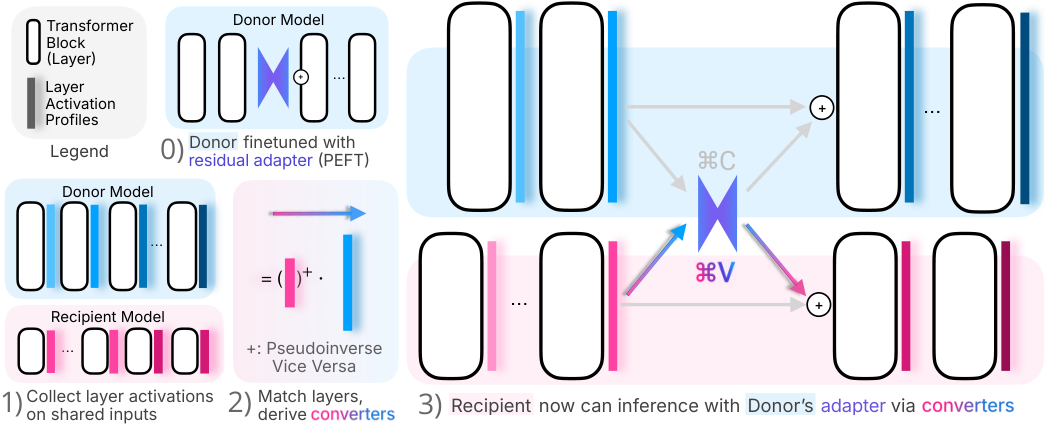
\includegraphics[width=0.99\linewidth]{figures/overview2.png}
\caption{Reusing PEFT weights on an architecturally different model with \cmdv{} requires little data and no backpropagation.
\cmdv{} can bring recipient models behaviors like jailbreaking prompt refusal.}
\label{fig:pipeline}
\end{figure}

Our contributions:
\begin{enumerate}
\item \textbf{Activation profiling.} A data-efficient method that establishes correspondences between residual neurons in distinct transformer LLMs.
\item \textbf{\cmdv{} adapter transfer.} Using activation profiles, we derive converters that paste new behaviors into a recipient without additional data or parameter updates.
\item \textbf{Effective behavior pasting.} On safety refusal, jailbreaking, and chain-of-thought prompting, \cmdv{} matches finetuning while using minimal compute.
\end{enumerate}

\obclaim{\cmdv{} matches or exceeds direct DiReFT on refusal, jailbreak, and auto-CoT while deriving converters in 6.35s on a laptop CPU and without the original training data.}
% OB-EDIT-END id=introduction


\section{Related Work}
\label{sec-related}
Our work intersects with model distillation, model merging, activation engineering, and parameter-efficient finetuning.

\paragraph{Knowledge distillation.}
Distillation~\cite{hinton2015,bucilua2006} trains a student to mimic a teacher's output probabilities or internal representations~\cite{romero2014}.
Standard distillation requires extensive teacher generation and significant student training.
\cmdv{} instead transfers the functional effect of a specific pre-existing adapter using activation mappings.

\paragraph{Model merging and editing.}
Merging typically assumes the same architecture and parameter count~\cite{wortsman2022,matena2022,yadav2023}.
Task arithmetic~\cite{ilharco2022} operates on finetuned weights.
ROME~\cite{meng2022rome} and MEMIT~\cite{meng2022memit} edit facts in weights.
\cmdv{} operates in activation space and transfers between distinct architectures.

\paragraph{Activation interpretability and engineering.}
Steering vectors added to residual outputs can adjust model behaviors~\cite{turner2023,zou2023repre,rimsky2024}.
Sparse linear features yield steering methods~\cite{gao2024,luo2024}.
Most of this work edits a single target model; \cmdv{} uses a donor's activations to steer a distinct recipient.

\paragraph{Parameter-efficient finetuning.}
Adapters~\cite{houlsby2019}, LoRA~\cite{hu2022lora}, and prefix-tuning~\cite{li2021prefix} add a small number of parameters.
Representation finetuning (ReFT)~\cite{wu2024reft} intervenes directly on hidden representations with low-rank projections.
\cmdv{} transfers DiReFT adapters from a donor without the PEFT training data.

\obtodo[id=cv-related, created=2025-02-03T10:00:00.000Z, updated=2025-06-02T09:33:41.000Z, completed=2025-06-02T09:33:41.000Z]{Separate distillation, merging, steering, and ReFT so the converter claim has a clean contrast.}

% OB-SECTION {"id":"method","label":"sec-method","level":2,"order":3,"title":"Computing and Using Activation Profiles"}

\section{Computing and Using Activation Profiles}
\label{sec-method}
% OB-EDIT-BEGIN openbarry/markdown@1 id=method
Let $M$ denote a transformer LLM with layers $L_m$ and hidden states $h_m^{\ell}\in\mathbb{R}^{d_m}$.
\cmdv{} uses three models: the donor $M_D$, a finetuned donor $M_{D'}$ that differs only by residual interventions, and the recipient $M_R$.
Let $P=\{p_1,\ldots,p_N\}$ be a set of prompts.

\paragraph{Algorithm.}
(1)~For each model $m\in\{D,R\}$ and layer $\ell_m$, store last-token activations of every $p_i$ as a matrix $A_m^{\ell_m}\in\mathbb{R}^{N\times d_m}$.
(2)~For each adapted donor layer $\ell_D$, match $\ell_R=\lfloor\alpha\cdot \ell_D\rfloor$ with $\alpha=|L_R|/|L_D|$, then set
$C_{R\to D}=(A_R^{\ell_R})^{\dagger}A_D^{\ell_D}$ and $C_{D\to R}=(A_D^{\ell_D})^{\dagger}A_R^{\ell_R}$.
(3)~At recipient inference, convert, apply $\Delta I^{\ell_D}$, convert back, and add:
$h^{\ell_R}\leftarrow h^{\ell_R}+C_{D\to R}\bigl(\Delta I^{\ell_D}(h^{\ell_R}C_{R\to D})\bigr)$.

\subsection{Activation profiling}

Following Zou et al.~\cite{zou2023repre}, we use last-token activations to match the adapter configuration.
For Llama-3.1-8B-Instruct ($d=4096$, 32 layers), $N=100$ prompts yield a $(100,4096)$ matrix per layer.
Intuitively, that matrix encodes how each residual dimension responds across diverse user prompts.

\obtodo[id=cv-lima-profiles, created=2025-02-18T09:10:00.000Z, updated=2025-03-04T21:16:08.000Z, completed=2025-03-04T21:16:08.000Z]{Capture last-token LIMA train activations, N=1030, batch 4, bfloat16, every layer of each model in Table 2.}

We use $N=1030$ prompts from the LIMA training split~\cite{zhou2023lima}.
The prompts cover open-ended questions, creative writing, and factual queries.
LIMA is easy to obtain and is not specialized to the downstream tasks---\cmdv{} does not depend on task-specific profiling data.
Activation profiles are task-agnostic and need only be built once per model.

\subsection{From activation profiles to representation transfer}

\paragraph{Representation adapters.}
We train DiReFT~\cite{wu2024reft} interventions that act on a frozen base model:
\begin{equation}
I(h)=h+W_2^{\top}(W_1 h+b),\qquad \Delta I(h)=I(h)-h.
\end{equation}
Rank is 8 in our experiments (the ReFT range is typically 4 to 32).
Every ReFT module intervenes only on selected prompt tokens, here last tokens, once per sequence rather than once per decoded token.
We train a module on every other donor layer, adding less than $0.04\%$ parameters.

\paragraph{Layer correspondence.}
Layer-specific functions tend to scale linearly with depth~\cite{tenney2019}.
We use
\begin{equation}
\ell_R=\lfloor\alpha\cdot \ell_D\rfloor\qquad\text{where}\qquad\alpha=|L_R|/|L_D|.
\end{equation}
MSE-minimizing matches collapse onto early recipient layers and contradict late-layer semantics; see Appendix~\ref{sec-appendix}.

\obtodo[id=cv-layer-match, created=2025-03-05T11:00:00.000Z, updated=2025-03-28T16:44:19.000Z, completed=2025-03-28T16:44:19.000Z]{Ablate linear depth matching against total-MSE layer assignment on Llama 3.1 8B to 3.2 3B.}
\obcomment[kind=result]{MSE matching dumps everything onto the earliest recipient layers and tanks downstream tasks. Keep the linear map.}

\paragraph{Layer converter.}
Let $X\in\mathbb{R}^{N\times d_R}$ and $Y\in\mathbb{R}^{N\times d_D}$ be paired last-token activations.
Least squares with the Moore-Penrose pseudoinverse gives
\begin{equation}
C_{R\to D}=X^{\dagger}Y,\qquad C_{D\to R}=Y^{\dagger}X.
\end{equation}
A bidirectional converter between Llama-3.2-3B ($d=3072$) and Llama-3.1-8B ($d=4096$) has shapes $(4096,3072)$ and $(3072,4096)$.
The maps are cycle-consistent in the least-squares sense and are computed on CPU.

\obtodo[id=cv-converters, created=2025-03-06T08:40:00.000Z, updated=2025-03-29T12:07:55.000Z, completed=2025-03-29T12:07:55.000Z]{Derive all layer-pair converters. Time the MacBook Pro CPU path.}
\obcomment[kind=result]{6.35s mean for 14--18 layer pairs on a MacBook Pro CPU. 3B-to-8B is 25.2M params per pair, 14 pairs, 352.8M converter params, still cheap vs backprop.}

\paragraph{Transfer mechanism.}
\begin{equation}
h^{{\ell_R},\mathrm{intervened}}=h^{\ell_R}+C_{D\to R}\bigl(\Delta I^{\ell_D}(C_{R\to D}(h^{\ell_R}))\bigr).
\end{equation}
If profiles already exist, an edge device can apply an 8B adapter to a 3B model without downloading the 8B weights.
Even when profiles must be built, the pass skips decoding and uses less peak memory than generation.
% OB-EDIT-END id=method


\section{Command-V in Practice}
\label{sec-experiments}
We port three behaviors chosen for large pre/post-finetuning gaps, easy verification, and practical utility: refusal enhancement, refusal suppression (jailbreak), and default chain-of-thought.

\paragraph{Adapter training.}
DiReFT on every other donor layer, last-token only, rank 8, 6 epochs, batch sizes 2 / 4 / 16 following Wu et al.~\cite{wu2024reft} Table~6 with those exceptions.

\subsection{Case study: refusal enhancement}

We train on 10,000 WildJailbreak~\cite{jiang2024} training prompts (harmful and benign adversarial).
Evaluation uses all 2,000 adversarial harmful and 221 adversarial benign prompts from the evaluation split.
LlamaGuard3 8B~\cite{grattafiori2024} labels harmful responses; we manually inspect benign overrefusal.

\obtodo[id=cv-refusal-train, created=2025-04-02T09:00:00.000Z, updated=2025-04-18T23:41:10.000Z, completed=2025-04-18T23:41:10.000Z]{Train DiReFT refusal adapters on Llama-3.1-8B and Llama-3.2-3B, WildJailbreak 10k, conservative batch 2/4.}
\obtodo[id=cv-refusal-eval, created=2025-04-19T10:15:00.000Z, updated=2025-04-27T14:08:33.000Z, completed=2025-04-27T14:08:33.000Z]{Plot ASR vs A100-40GB wall time for ReFT checkpoints and Command-V, including amortized profiling cost.}

A completed 3B adapter drops test ASR from $31.30\%$ to $12.20\%$ (intermediary low $5.65\%$).
Ported onto 8B, ASR falls $36.85\%\to 20.40\%$, beating direct 8B ReFT ($28.55\%$, intermediary low $21.05\%$).
The reverse 8B$\to$3B paste reaches $16.4\%$ ASR (Figure~\ref{fig:refusal}).

\begin{figure}[t]
\centering
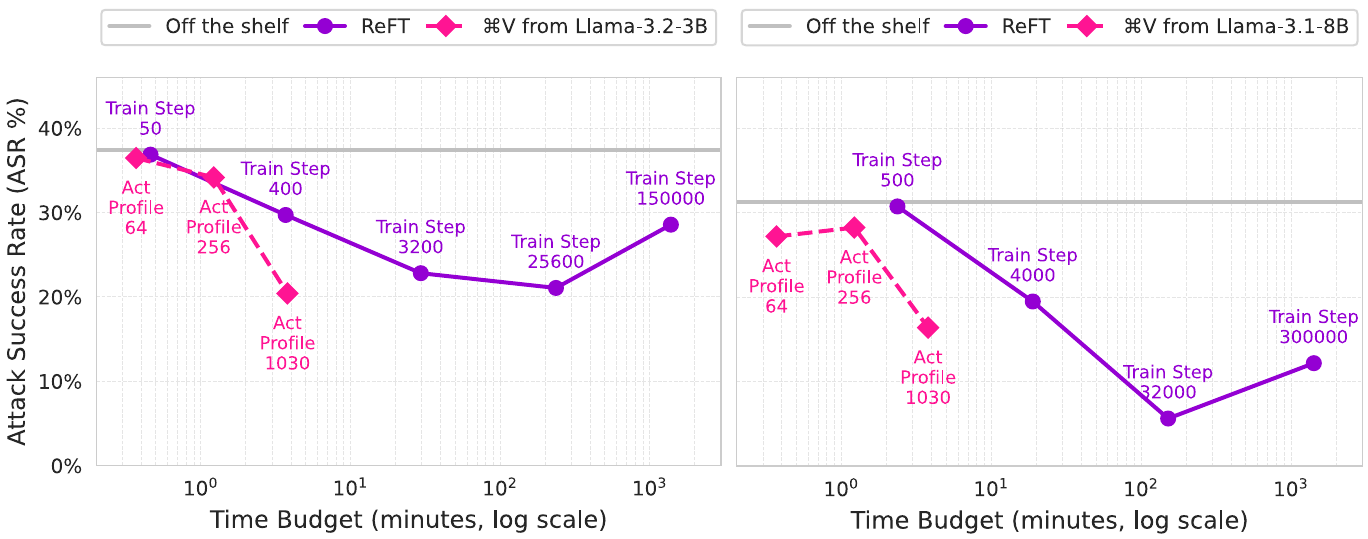
\includegraphics[width=\linewidth]{figures/WildJailbreak.png}
\caption{Reduced jailbreak attack success rate (ASR $\downarrow$) on Llama-3.2-3B-Instruct (left) and Llama-3.1-8B-Instruct (right).
Purple: WildJailbreak ReFT. Pink: \cmdv{}.
\cmdv{} sits on the cost--performance Pareto frontier. Time is A100 40GB wall time.}
\label{fig:refusal}
\end{figure}

\obcomment[kind=result]{3B adapter pasted onto 8B beats training the 8B adapter directly (20.40 vs 28.55 ASR). Keep that as the teaser number. Larger ReFT batches (12/16) trained faster and defended worse --- do not quote those.}

\paragraph{Overrefusal.}
Undesirable refusals on jailbreak-shaped but legitimate queries increase with ReFT and more with \cmdv{} (Table~\ref{tab:overrefusal}).

\begin{table}[t]
\centering
\caption{Human-annotated overrefusal rate ($\downarrow$) on WildJailbreak adversarial-benign test prompts.}
\label{tab:overrefusal}
\begin{tabular}{lccc}
\toprule
Model & Off-shelf (\%) & ReFT (\%) & \cmdv{} (\%) \\
\midrule
Llama 3.1 8B & 1.36 & 2.26 & 4.52 \\
Llama 3.2 3B & 3.17 & 8.60 & 14.48 \\
\bottomrule
\end{tabular}
\end{table}

\obtodo[id=cv-overrefusal, created=2025-04-28T13:00:00.000Z, updated=2025-05-06T19:22:47.000Z, completed=2025-05-06T19:22:47.000Z]{Human-label overrefusal on the 221 adversarial-benign prompts for off-shelf, ReFT, and Command-V.}

\paragraph{Efficiency.}
Profiling is a forward pass, amortized per model.
Converters take 6.35s mean on a MacBook Pro CPU for 14--18 layer pairs.

\subsection{Case study: refusal suppression}

Train and evaluate on AdvBench~\cite{zou2023advbench}; transfer-check on HarmBench Standard~\cite{mazeika2024}.
LlamaGuard3 8B is the safety classifier.
We port across Llama~3, Qwen2.5, and Gemma~2 instruct models, and additionally run inference-only recipients Phi-4-mini and OLMo~2 (not trainable in the ReFT library at the time).

\obtodo[id=cv-jailbreak-matrix, created=2025-05-07T09:30:00.000Z, updated=2025-05-28T02:17:09.000Z, completed=2025-05-28T02:17:09.000Z]{Fill the AdvBench and HarmBench donor-recipient ASR heatmaps, including same-family boxes.}

\begin{figure}[hpt]
\centering
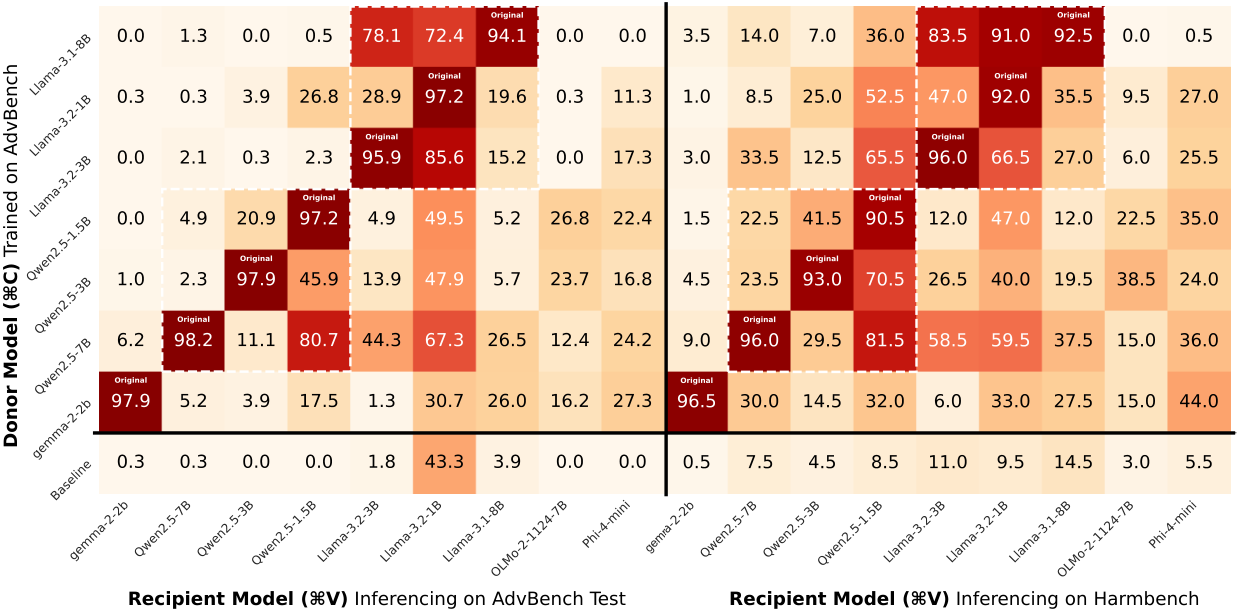
\includegraphics[width=0.99\linewidth]{figures/grid.png}
\caption{Jailbreaking and \cmdv{}: porting jailbreakability often increases ASR ($\uparrow$), especially in the same model family (white dashed boxes).
Diagonal entries are ReFT adapter validation performance, an upper bound on expected \cmdv{} transfer.
All models are instruct versions.}
\label{fig:grid}
\end{figure}

Off-shelf models sit at single-digit ASR (Figure~\ref{fig:grid}).
After \cmdv{}, many jump to $20$--$80\%$.
Qwen2.5-7B-Instruct is the best donor: mean $41.2\%$ AdvBench and $46.9\%$ HarmBench when ported, up to $80.7\%$ / $81.5\%$ on Qwen2.5-1.5B-Instruct.
Llama-3.2-1B-Instruct is the most susceptible recipient (mean $61.7\%$ / $54.9\%$).
Gemma2-2B-it is the most resistant: no donor jailbreaks it meaningfully.
Same-family transfers dominate the heatmaps.
LIMA profiles were not collected on harmful prompts and still transferred.

\obcomment[kind=result]{Qwen2.5-7B donor is the jailbreak workhorse. Gemma2-2B-it refused every paste. Put both in the caption so the heatmap is not read as universal transfer.}

\subsection{Case study: increased use of chain-of-thought}

We train ReFT on 2,000 OpenMathReasoning~\cite{moshkov2025} examples, replacing specialized thinking delimiter tokens with natural words to avoid tokenizer-mismatch garbage after porting.
Evaluation: two Big-Bench Hard~\cite{suzgun2022} tasks with the largest original CoT lifts, 250 test questions each, answers requested as short JSON.

\obtodo[id=cv-cot-openmath, created=2025-05-12T10:00:00.000Z, updated=2025-06-09T18:51:26.000Z, completed=2025-06-09T18:51:26.000Z]{Port OpenMathReasoning CoT adapters across Qwen2.5 and Llama 3.1/3.2 sizes on BBH multistep arithmetic and tracking shuffled objects.}

\begin{figure}[h]
\centering
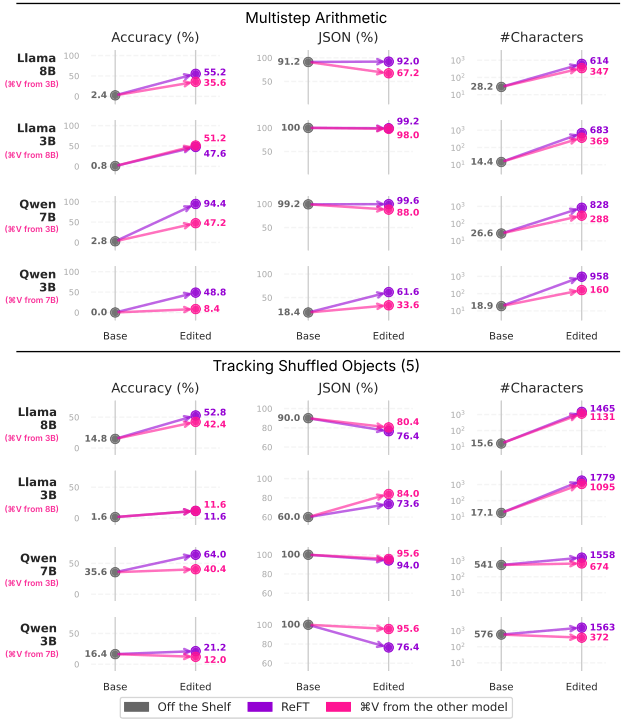
\includegraphics[width=0.85\linewidth]{figures/reasoning2.png}
\caption{Trained and \cmdv{} performance on Big-Bench Hard.
Same-family OpenMathReasoning ports increase output length and task accuracy, comparable to direct ReFT, while more responses fail the requested JSON format (middle column).}
\label{fig:cot}
\end{figure}

JSON makes extraction easy and depresses absolute accuracy relative to unconstrained decoding (Figure~\ref{fig:cot}).
Multistep arithmetic sees marked gains; Qwen2.5-3B is the largest porting lift ($+50\%$).
Tracking shuffled objects is a smaller but real lift, especially on larger models.
Reasoning quality improved uniformly; instruction following sometimes collapsed, with up to $28.8\%$ of responses failing the JSON format, plus occasional language drift on Qwen.

\obcomment[kind=result]{CoT paste works as more characters and higher task accuracy, with a format-collapse tax. Do not bury the 28.8 percent JSON failure --- it is the honest limitation next to the +50 percent Qwen 3B lift.}

% OB-SECTION {"id":"discussion","label":"sec-discussion","level":2,"order":5,"title":"Discussion"}

\section{Discussion}
\label{sec-discussion}
% OB-EDIT-BEGIN openbarry/markdown@1 id=discussion
These results are a proof of concept that behaviors can be ported across models.
Natural next steps, beyond this paper, include pasting English-data instruction following into a low-resource-language model, composing several specialist adapters into one recipient, and replacing least-squares converters with nonlinear or trained maps.

\cmdv{} is not useful when the donor adapter itself barely moves the donor.
Finetuning on a commonsense ReFT setup~\cite{hu2023adapters,wu2024reft} or on TOFU fictitious knowledge~\cite{maini2024} gave modest donor gains and negligible recipient gains.

\obtodo[id=cv-failed-tasks, created=2025-05-20T11:40:00.000Z, updated=2025-06-11T09:12:04.000Z, completed=2025-06-11T09:12:04.000Z]{Record the commonsense ReFT and TOFU negative transfers so Discussion does not overclaim.}
\obcomment[kind=result]{If the donor adapter is weak, Command-V is a no-op. That is a method limit, not a missing ablation.}

Recipient utility can also collapse after a paste, especially on smaller models, similar to activation oversteering~\cite{konen2024}.
Exact token formats such as specialized thinking delimiters become confused or malformed.
Llama 3.2 3B and 3.1 8B are empirically better transfer partners than others; predicting good pairs remains open.
Jailbreaking transfers across families more readily than refusal enhancement or reasoning.

Even with those limits, \cmdv{} is Pareto-optimal on cost versus performance for the behaviors that do transfer: no task-specific data, and orders of magnitude less compute than training the recipient adapter.

\paragraph{Broader impact.}
The method is meant for generic task finetuning and helps beneficial behaviors such as safety refusal.
Because it also ports jailbreaking cheaply, it could lower the barrier to using open-weight models for harmful requests.
At publication we are not adding a new vulnerability beyond adapters and jailbreak prompts already on the internet.

\obtodo[id=cv-discussion, created=2025-06-10T14:00:00.000Z, updated=2025-06-16T10:28:51.000Z, completed=2025-06-16T10:28:51.000Z]{Write limitations, negative transfers, and the jailbreak broader-impact paragraph.}
\obtodo[id=cv-arxiv, created=2025-06-20T09:00:00.000Z, updated=2025-06-23T18:04:00.000Z, completed=2025-06-23T18:04:00.000Z]{arXiv 2506.19140 plus public GitHub snapshot.}
\obtodo[id=cv-code-release, created=2025-06-15T16:00:00.000Z, updated=2025-06-23T18:10:00.000Z, completed=2025-06-23T18:10:00.000Z]{Release step1/2/3 scripts, LIMA profiles instructions, and the demo notebook.}
\obtodo[id=cv-iclr, created=2025-09-18T12:00:00.000Z, updated=2025-09-24T21:16:44.000Z, completed=2025-09-24T21:16:44.000Z]{ICLR 2026 OpenReview submit (forum oRYzpI3cmJ).}
\obtodo[id=cv-camera, created=2026-01-28T15:00:00.000Z, updated=2026-02-12T11:37:08.000Z, completed=2026-02-12T11:37:08.000Z]{Camera-ready: reviewer notes on overrefusal, JSON collapse, and Gemma2-2B resistance.}
% OB-EDIT-END id=discussion


\section{Acknowledgements}
\label{sec-ack}
This research was supported by a sponsorship from Cisco (BW, DI).
We also thank Google for providing inference and compute services with credits.

\begin{thebibliography}{99}
\bibitem{hu2022lora} Hu, Edward J. et al. LoRA: Low-rank adaptation of large language models. ICLR 2022.
\bibitem{wei2021flan} Wei, Jason et al. Finetuned Language Models are Zero-Shot Learners. 2021.
\bibitem{christiano2017} Christiano, Paul F. et al. Deep Reinforcement Learning from Human Preferences. NeurIPS 2017.
\bibitem{xia2024} Xia, Y. et al. Understanding the Performance and Estimating the Cost of LLM Fine-Tuning. IISWC 2024.
\bibitem{hinton2015} Hinton, Geoffrey, Oriol Vinyals, and Jeff Dean. Distilling the Knowledge in a Neural Network. 2015.
\bibitem{bucilua2006} Bucilu{\v{a}}, Cristian, Rich Caruana, and Alexandru Niculescu-Mizil. Model Compression. KDD 2006.
\bibitem{romero2014} Romero, Adriana et al. FitNets: Hints for Thin Deep Nets. 2014.
\bibitem{wortsman2022} Wortsman, Mitchell et al. Model soups. ICML 2022.
\bibitem{matena2022} Matena, Michael S. and Colin A. Raffel. Merging Models with Fisher-Weighted Averaging. NeurIPS 2022.
\bibitem{yadav2023} Yadav, Prateek et al. TIES-Merging. NeurIPS 2023.
\bibitem{ilharco2022} Ilharco, Gabriel et al. Editing Models with Task Arithmetic. 2022.
\bibitem{meng2022rome} Meng, Kevin et al. Locating and Editing Factual Associations in GPT. NeurIPS 2022.
\bibitem{meng2022memit} Meng, Kevin et al. Mass-Editing Memory in a Transformer. 2022.
\bibitem{turner2023} Turner, Alexander Matt et al. Activation Addition. 2023.
\bibitem{zou2023repre} Zou, Andy et al. Representation Engineering. 2023.
\bibitem{rimsky2024} Rimsky, Nina et al. Steering Llama 2 via Contrastive Activation Addition. ACL 2024.
\bibitem{gao2024} Gao, Leo et al. Scaling and evaluating sparse autoencoders. 2024.
\bibitem{luo2024} Luo, Jinqi et al. PaCE. NeurIPS 2024.
\bibitem{houlsby2019} Houlsby, Neil et al. Parameter-Efficient Transfer Learning for NLP. ICML 2019.
\bibitem{li2021prefix} Li, Xiang Lisa and Percy Liang. Prefix-Tuning. 2021.
\bibitem{wu2024reft} Wu, Zhengxuan et al. ReFT: Representation Finetuning for Language Models. NeurIPS 2024.
\bibitem{zhou2023lima} Zhou, Chunting et al. LIMA: Less Is More for Alignment. NeurIPS 2023.
\bibitem{tenney2019} Tenney, Ian, Dipanjan Das, and Ellie Pavlick. BERT Rediscovers the Classical NLP Pipeline. ACL 2019.
\bibitem{tenney2019b} Tenney, Ian et al. What Do You Learn from Context? 2019.
\bibitem{grattafiori2024} Grattafiori, Aaron et al. The Llama 3 Herd of Models. 2024.
\bibitem{jiang2024} Jiang, Liwei et al. WildTeaming at Scale. NeurIPS 2024.
\bibitem{zou2023advbench} Zou, Andy et al. Universal and Transferable Adversarial Attacks on Aligned Language Models. 2023.
\bibitem{mazeika2024} Mazeika, Mantas et al. HarmBench. 2024.
\bibitem{moshkov2025} Moshkov, Ivan et al. OpenMathReasoning. 2025.
\bibitem{suzgun2022} Suzgun, Mirac et al. Challenging BIG-Bench Tasks and Whether Chain-of-Thought Can Solve Them. 2022.
\bibitem{hu2023adapters} Hu, Zhiqiang et al. LLM-adapters. EMNLP 2023.
\bibitem{maini2024} Maini, Pratyush et al. TOFU. 2024.
\bibitem{konen2024} Konen, Kai et al. Style Vectors for Steering Generative Large Language Models. 2024.
\end{thebibliography}

\appendix

\section{Additional Details}
\label{sec-appendix}
\subsection{Activation profile setup}

We forward 1030 LIMA~\cite{zhou2023lima} prompts in order and capture last-prompt-token activations at every transformer-layer output, default generation parameters, no hyperparameter search.
Batch size 4, activations stored in bfloat16.

\subsection{Layer matching}

MSE-guided matching overwhelmingly assigns donor layers to the earliest possible recipient layers (Figure~\ref{fig:llama-mse}).
That disagrees with evidence that semantic functions concentrate in late layers~\cite{tenney2019b} and does not transfer well.
Linear depth matching is the default in the main experiments.

\begin{figure}[htbp]
\centering
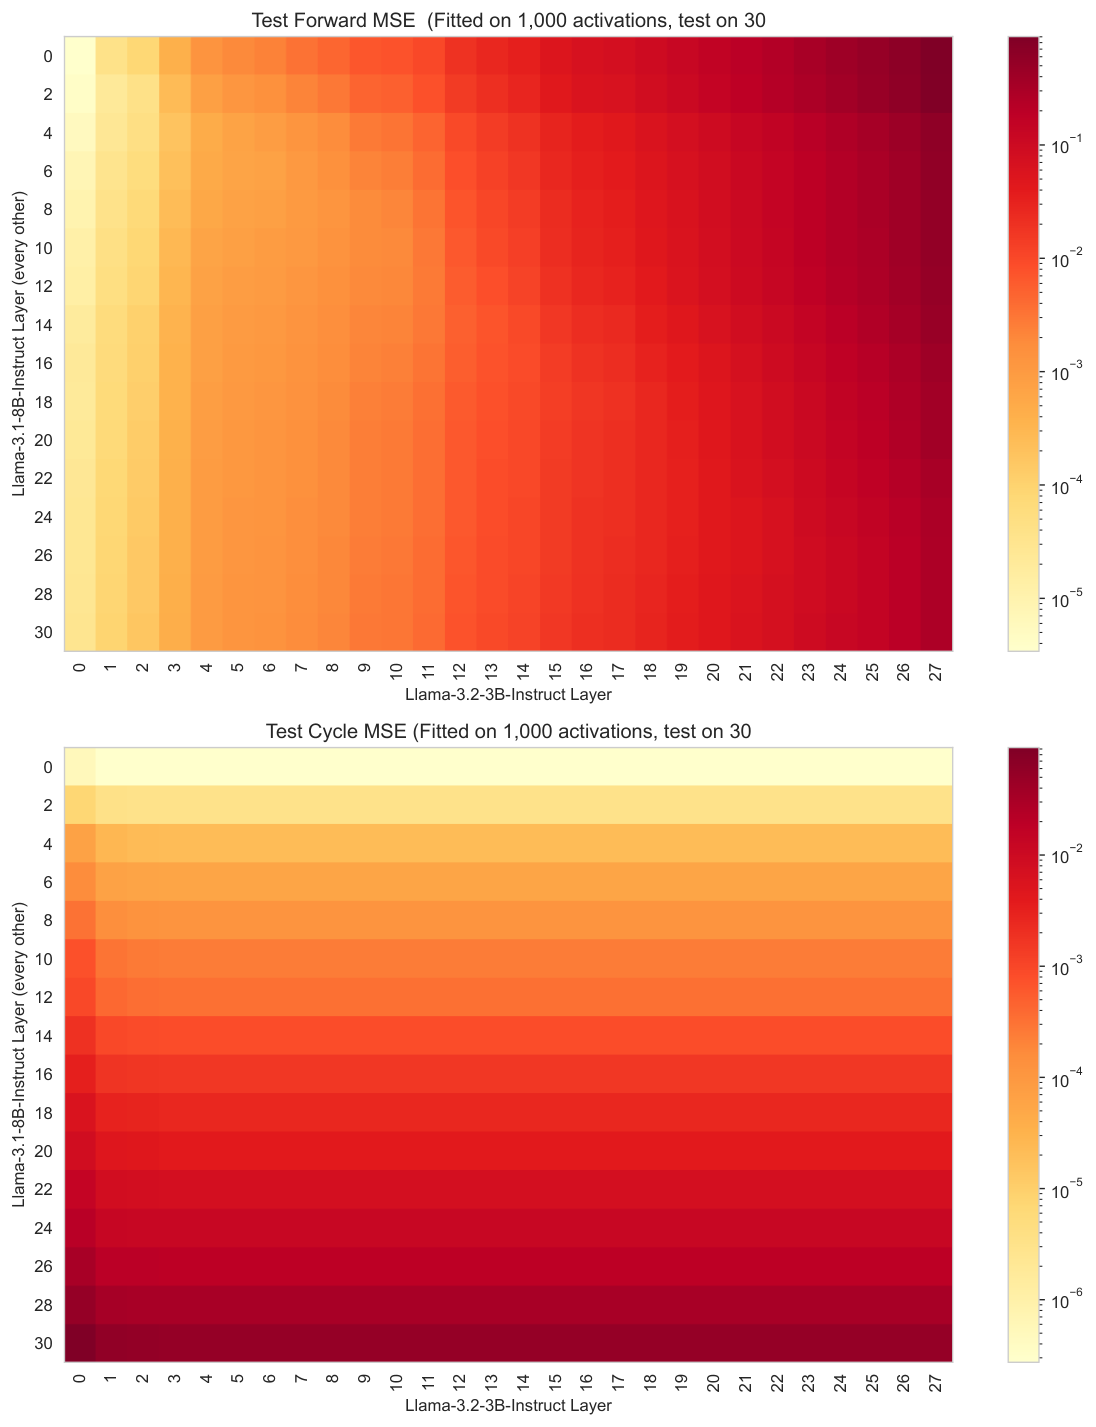
\includegraphics[width=0.8\linewidth]{figures/llama_detailed_analysis.png}
\caption{Llama-3.1-8B-Instruct to Llama-3.2-3B-Instruct test loss, averaged across input.
Minimizing forward or cycle loss is a poor layer-mapping strategy because later layers are harder to reconstruct.}
\label{fig:llama-mse}
\end{figure}

\subsection{Models}

All instruct checkpoints from Hugging Face as of March 2025.

\begin{table}[h]
\centering
\small
\caption{Language models used in experiments.}
\label{tab:models}
\begin{tabular}{lcccc}
\toprule
Model & Release & Size & Depth & Hidden \\
\midrule
Llama-3.1-8B-Instruct & 2024-07 & 8B & 32 & 4096 \\
Llama-3.2-3B-Instruct & 2024-09 & 3B & 28 & 3072 \\
Llama-3.2-1B-Instruct & 2024-09 & 1B & 16 & 2048 \\
Qwen2.5-7B-Instruct & 2024-09 & 7B & 28 & 4096 \\
Qwen2.5-3B-Instruct & 2024-09 & 3B & 36 & 2560 \\
Qwen2.5-1.5B-Instruct & 2024-09 & 1.5B & 28 & 2048 \\
Gemma-2-2B-it & 2024-05 & 2B & 26 & 2304 \\
Phi-4-mini-instruct & 2025-02 & 3.8B & 32 & 3072 \\
OLMo-2-1124-7B-Instruct & 2024-11 & 7B & 32 & 4096 \\
\bottomrule
\end{tabular}
\end{table}

Parameter count per layer pair is $2\,d_R d_D$.
Example: 3B$\leftrightarrow$8B is $2\times 3072\times 4096=25.2$M per pair.
Fourteen pairs: $352.8$M converter parameters, still MFLOPs added per token relative to the base forward pass.

\subsection{Converter reconstruction error}

Forward and cycle MSE between profiled last-token activations is low within family and higher across Gemma$\leftrightarrow$Qwen than Llama$\leftrightarrow$Llama (Figure~\ref{fig:converter-mse}), consistent with the jailbreak heatmap (same-family boxes transfer, Gemma2-2B resists).

\begin{figure}[htbp]
\centering
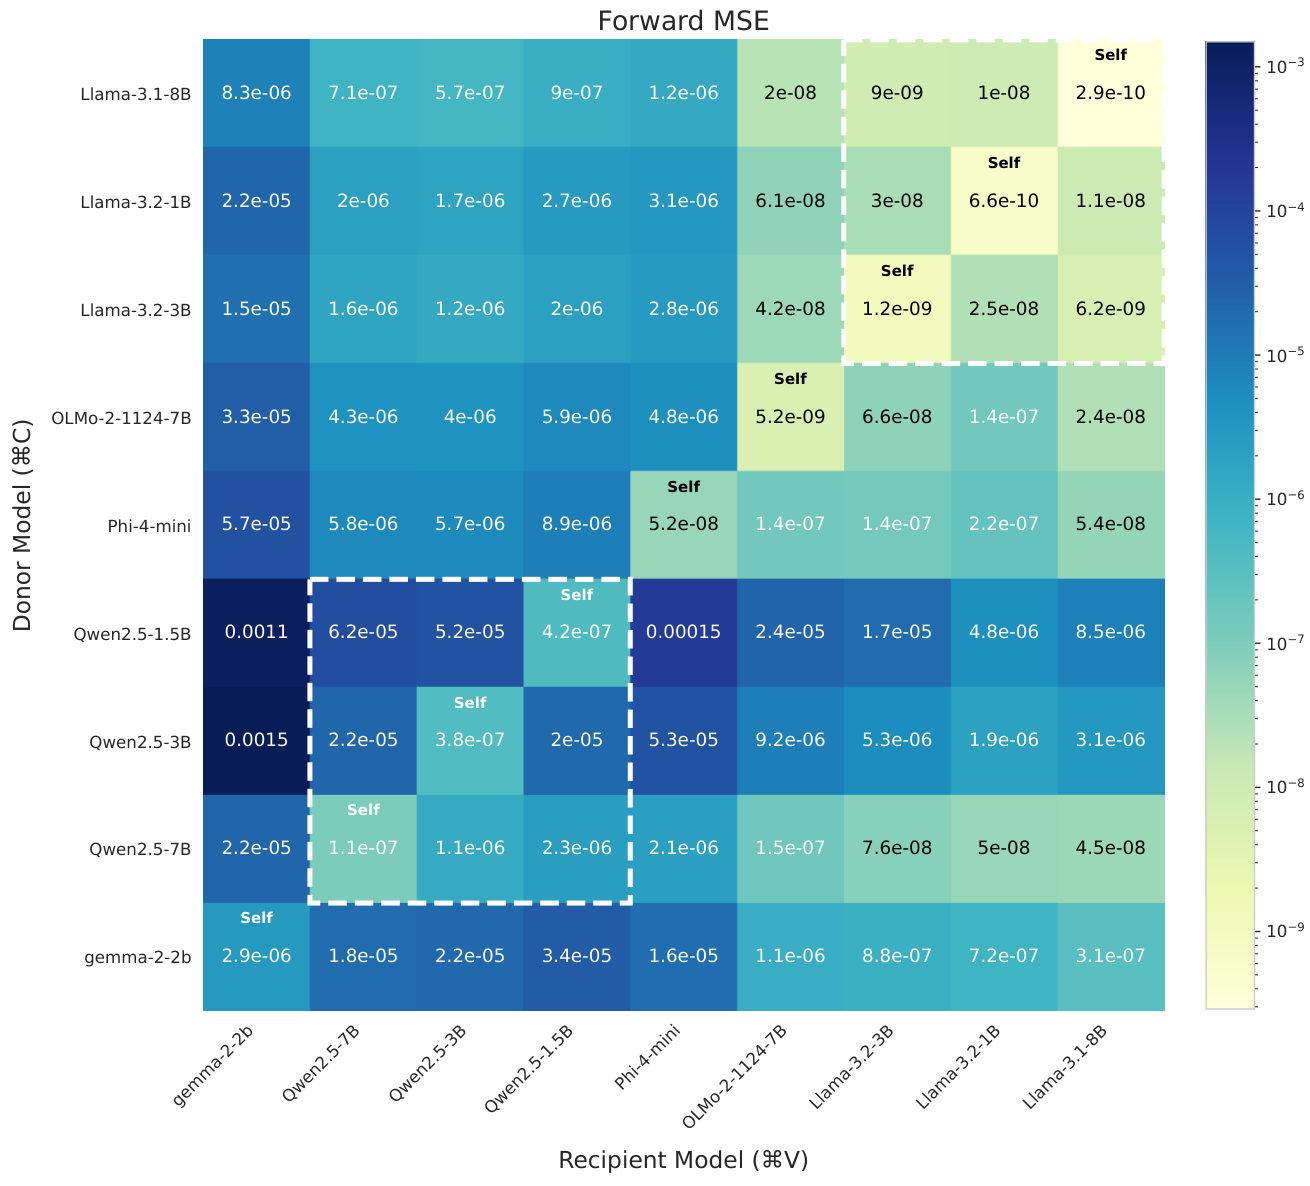
\includegraphics[width=0.8\linewidth]{figures/correlations_pseudoinverse1.png}

\vspace{0.6em}
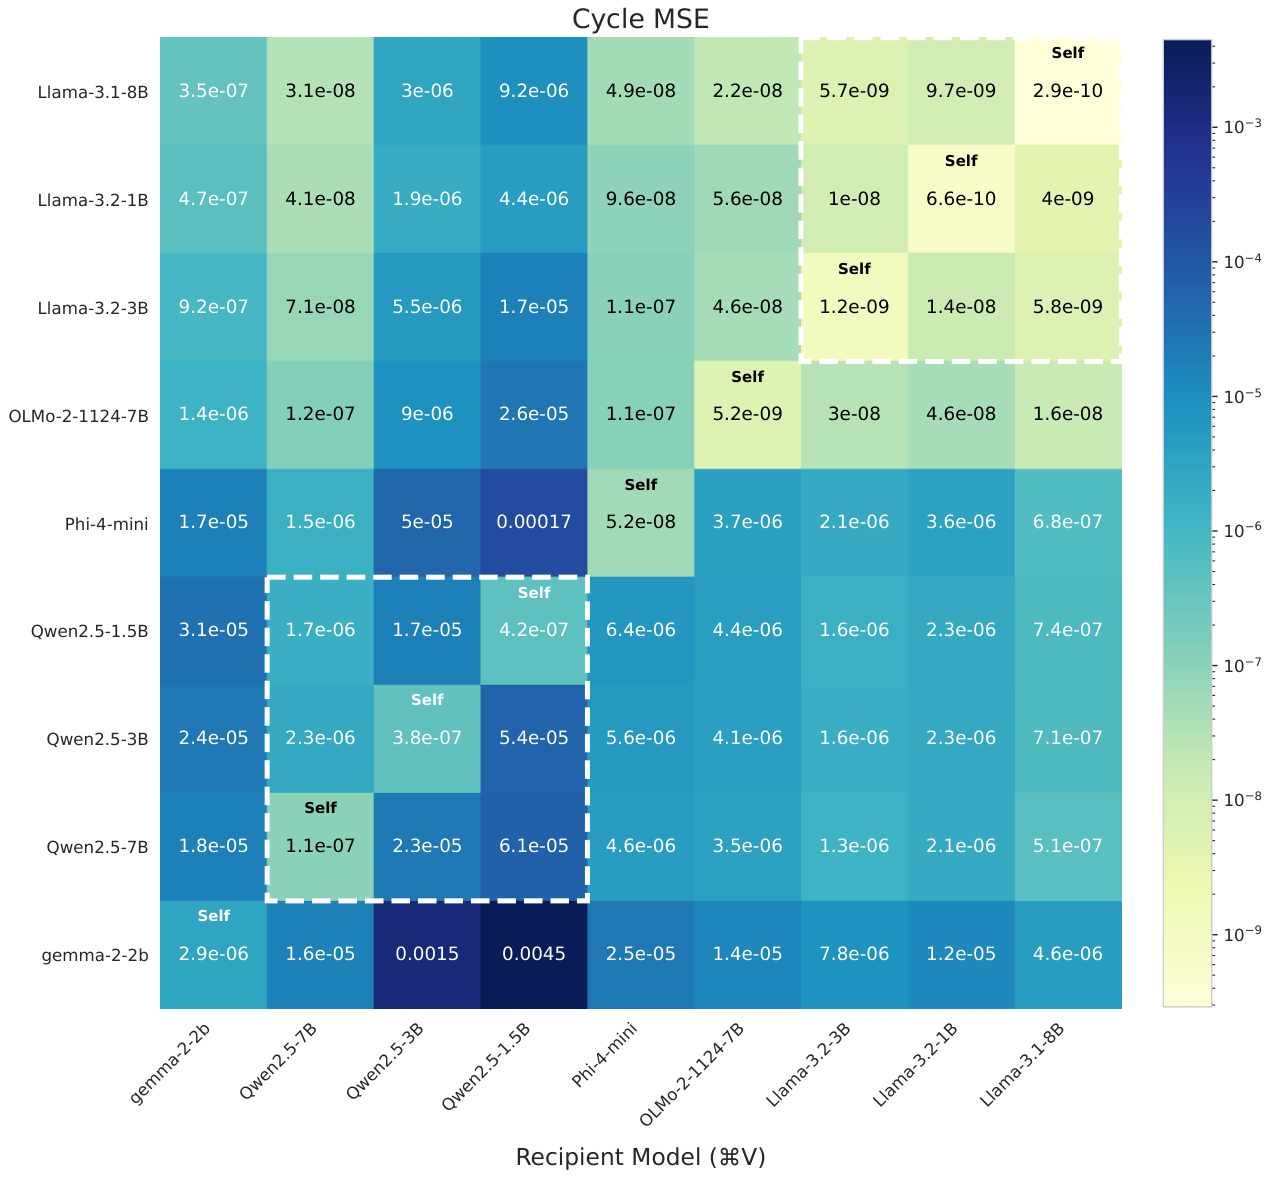
\includegraphics[width=0.8\linewidth]{figures/correlations_pseudoinverse2.png}
\caption{Forward (top) and cycle (bottom) training MSE of pseudoinverse residual-layer converters.
Same-family pairs are marked with a white square.
Values are unnormalized, so only entries in the same column (recipient) of the top plot and the same row (donor) of the bottom plot are comparable.}
\label{fig:converter-mse}
\end{figure}

\subsection{Converter wall time}

Deriving converters takes seconds on a laptop CPU once activation profiles exist (Figure~\ref{fig:converter-time}).

\begin{figure}[htbp]
\centering
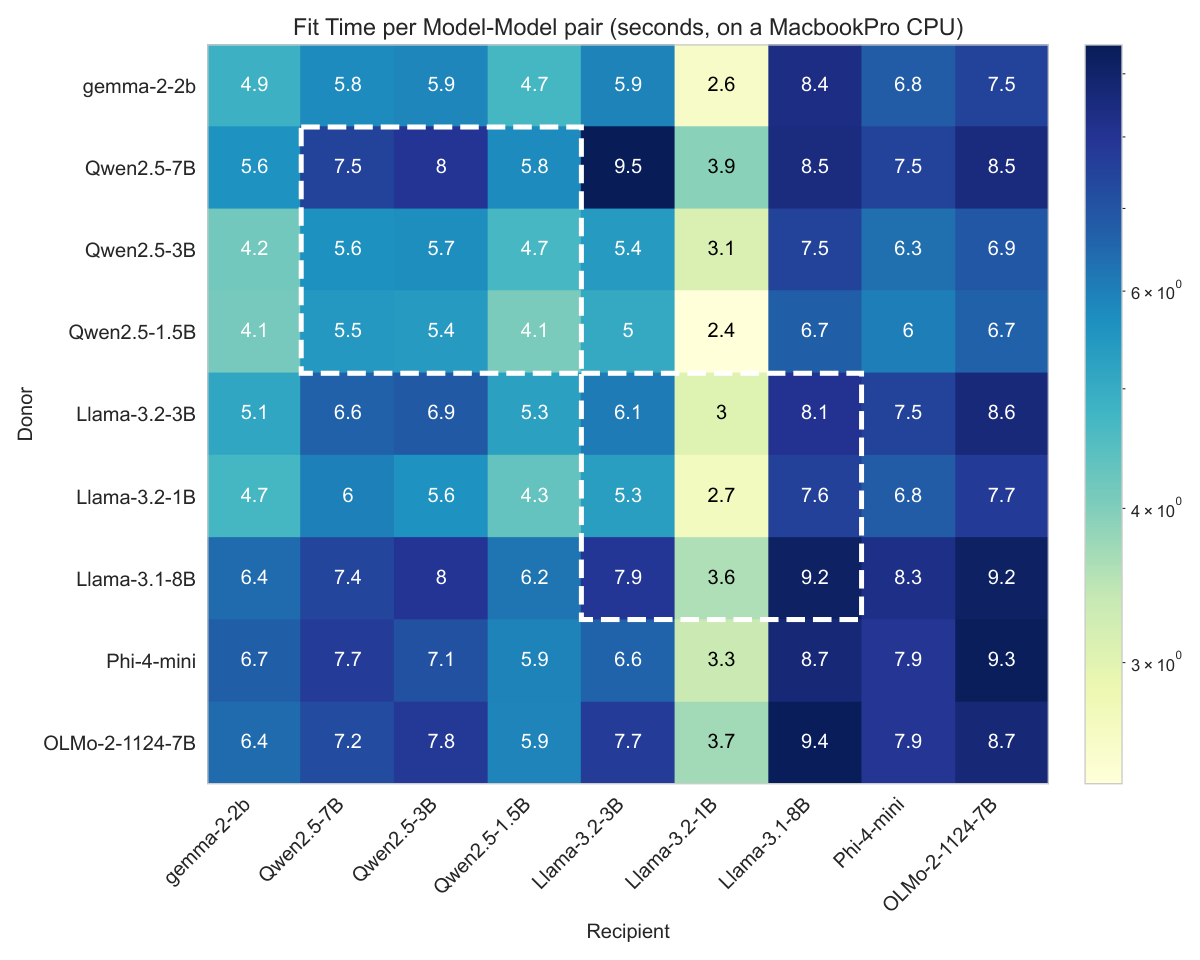
\includegraphics[width=0.8\linewidth]{figures/converter_time.png}
\caption{Pseudoinverse converter deriving time per model pair on an M1 Max CPU.}
\label{fig:converter-time}
\end{figure}

\end{document}
